% UML stavový diagram pipeline auditu jedného modelu.
% Samostatne: latexmk -pdf pipeline.tex   V dokumentácii: \includestandalone{uml/pipeline}
\documentclass[tikz,border=4pt]{standalone}
\usepackage[T1]{fontenc}
\usepackage{lmodern}
\usetikzlibrary{arrows.meta,positioning,shapes.geometric,shapes.multipart}
\begin{document}
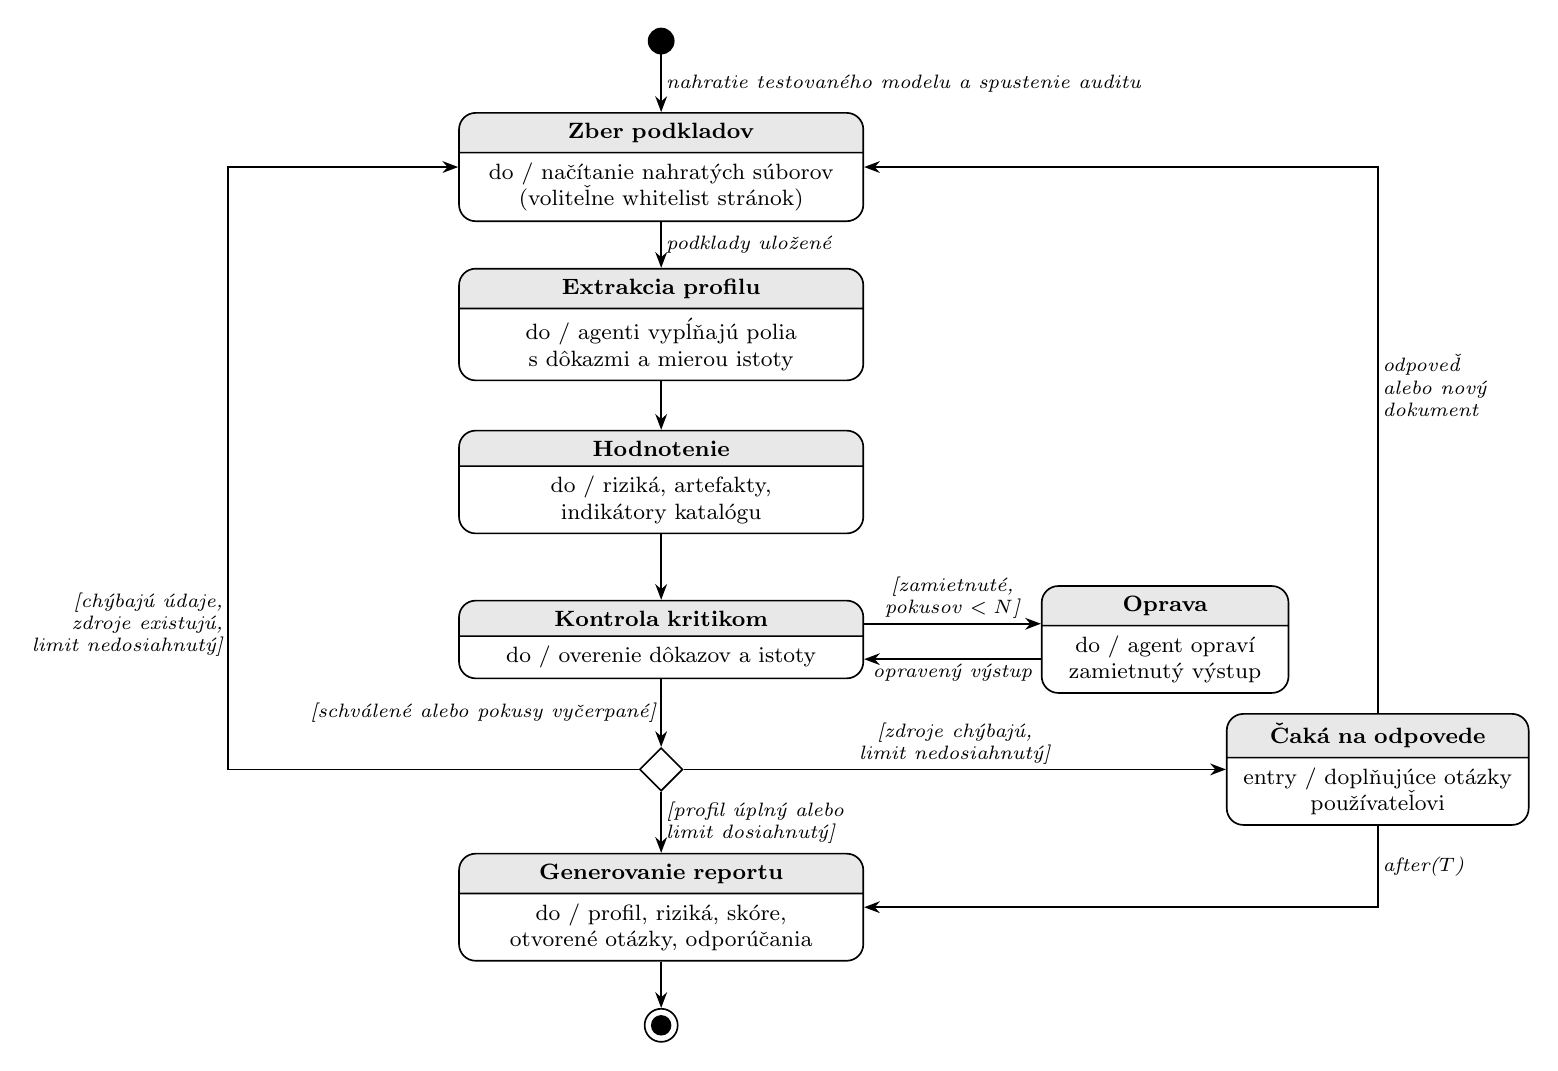
\begin{tikzpicture}[
    font=\footnotesize,
    % UML stav: zaoblený obdĺžnik s názvom a vnútornou aktivitou
    stav/.style={draw, rounded corners=6pt, rectangle split, rectangle split parts=2,
        rectangle split part fill={gray!18, white}, text width=4.9cm, align=center, semithick},
    cakanie/.style={stav, text width=3.6cm},
    volba/.style={draw, diamond, minimum size=0.55cm, inner sep=0pt, fill=white, semithick},
    prechod/.style={-{Stealth[length=2mm]}, semithick},
    popis/.style={font=\scriptsize\itshape, inner sep=1.5pt}
]
    \fill (6.5,0.4) circle (0.17cm) coordinate (init);
    \node[stav] (zber) at (6.5,-1.2) {\textbf{Zber podkladov}\nodepart{second}do / načítanie nahratých súborov\\(voliteľne whitelist stránok)};
    \node[stav] (extr) at (6.5,-3.2) {\textbf{Extrakcia profilu}\nodepart{second}do / agenti vypĺňajú polia\\s~dôkazmi a~mierou istoty};
    \node[stav] (hodn) at (6.5,-5.2) {\textbf{Hodnotenie}\nodepart{second}do / riziká, artefakty,\\indikátory katalógu};
    \node[stav] (krit) at (6.5,-7.2) {\textbf{Kontrola kritikom}\nodepart{second}do / overenie dôkazov a~istoty};
    \node[volba] (v) at (6.5,-8.85) {};
    \node[stav, text width=2.9cm] (oprava) at (12.9,-7.2) {\textbf{Oprava}\nodepart{second}do / agent opraví\\zamietnutý výstup};
    \node[cakanie] (caka) at (15.6,-8.85) {\textbf{Čaká na odpovede}\nodepart{second}entry / doplňujúce otázky\\používateľovi};
    \node[stav] (rep) at (6.5,-10.6) {\textbf{Generovanie reportu}\nodepart{second}do / profil, riziká, skóre,\\otvorené otázky, odporúčania};
    \node[circle, draw, semithick, minimum size=0.42cm, inner sep=0pt] (fin) at (6.5,-12.1) {};
    \fill (fin) circle (0.13cm);

    \draw[prechod] (0,0.4 -| init) ++(0,-0.17) -- node[popis, right] {nahratie testovaného modelu a~spustenie auditu} (zber);
    \draw[prechod] (zber) -- node[popis, right] {podklady uložené} (extr);
    \draw[prechod] (extr) -- (hodn);
    \draw[prechod] (hodn) -- (krit);
    \draw[prechod] (krit) -- node[popis, left] {[schválené alebo pokusy vyčerpané]} (v);

    % zamietnutý výstup opraví ten agent, ktorý ho vytvoril (extrakcia aj hodnotenie)
    \draw[prechod] ([yshift=0.2cm]krit.east) -- node[popis, above, align=center] {[zamietnuté,\\pokusov $<N$]} ([yshift=0.2cm]krit.east -| oprava.west);
    \draw[prechod] ([yshift=-0.25cm]krit.east -| oprava.west) -- node[popis, below] {opravený výstup} ([yshift=-0.25cm]krit.east);
    % chýbajúce údaje, ktoré sa dajú dohľadať
    \draw[prechod] (v.west) -- (1.0,-8.85) |- node[popis, pos=0.12, left, align=right] {[chýbajú údaje,\\zdroje existujú,\\limit nedosiahnutý]} (zber.west);
    % zdroje chýbajú: doplňujúce otázky
    \draw[prechod] (v.east) -- node[popis, above, align=center] {[zdroje chýbajú,\\limit nedosiahnutý]} (caka.west);
    \draw[prechod] (caka.north) |- node[popis, pos=0.3, right, align=left] {odpoveď\\alebo nový\\dokument} (zber.east);
    \draw[prechod] (v) -- node[popis, right, align=left] {[profil úplný alebo\\limit dosiahnutý]} (rep);
    % používateľ neodpovedá: audit sa ukončí, otázky zostanú v reporte ako otvorené
    \draw[prechod] (caka.south) |- node[popis, pos=0.25, right, align=left] {after($T$)} (rep.east);
    \draw[prechod] (rep) -- (fin);
\end{tikzpicture}
\end{document}
